\documentclass[10pt,twocolumn,letterpaper]{article}
\usepackage[affil-it]{authblk}
\usepackage{blindtext}
\usepackage{abstract}

\usepackage{iccv}
\iccvfinalcopy
\def\iccvPaperID{}
\usepackage[utf8]{inputenc}
\usepackage{parskip}
\usepackage{tcolorbox}
\usepackage{pdfpages}
\newcommand*{\quedb}{\hfill\ensuremath{\square}}%
\usepackage{anyfontsize}
\usepackage{linguex}
\usepackage{mathtools}
\usepackage[hang]{footmisc}

\definecolor{pink}{HTML}{EC008C}
\usepackage{times}
\usepackage{graphicx}
\usepackage{xcolor}
\usepackage[colorlinks = true,
            linkcolor = pink,
            urlcolor  = pink,
            citecolor = pink,
            anchorcolor = pink]{hyperref}
            
\usepackage{amssymb}

% additional packages
\usepackage{amsmath}
\usepackage{bbm}
\usepackage{support-caption}
\usepackage{subcaption}
\usepackage{tikz, tikz-3dplot} 
\usetikzlibrary{calc}
\usetikzlibrary{matrix}
\usepackage{url}
\renewcommand{\footnotesize}{\fontsize{7.5pt}{7.5pt}\selectfont}
\setlength{\footnotemargin}{0mm}

\usepackage{float}
\usepackage{amsthm}
\usepackage{booktabs}

%% local defs
% macros
\newtheorem{theorem}{Theorem}
\newtheorem{lemma}[theorem]{Lemma}
\newtheorem{proposition}[theorem]{Proposition}
\newcommand{\norm}[1]{\left\lVert#1\right\rVert}
\providecommand{\keywords}[1]{\textbf{\textit{Author Keywords:}} #1}

% confusion matrix
\usepackage{array}
\usepackage{multirow}

\newcommand\MyBox[2]{
  \fbox{\lower0.75cm
    \vbox to 1.7cm{\vfil
      \hbox to 1.7cm{\hfil\parbox{1.4cm}{#1\\#2}\hfil}
      \vfil}%
  }%
}

\usepackage{tikzpagenodes}

\title{A Simple Machine Learning Framework to Aid Citation Screening in
Systematic Reviews and Meta-Analyses of Aging and Longevity Research Studies}
\author{%
	Marko Lalović\thanks{\footnotesize{%
	\url{mailto:marko@markolalovic.com}%
	}}
}

\begin{document}

\twocolumn[{%
\renewcommand\twocolumn[1][]{#1}%
\maketitle
\begin{center}
    \centering
    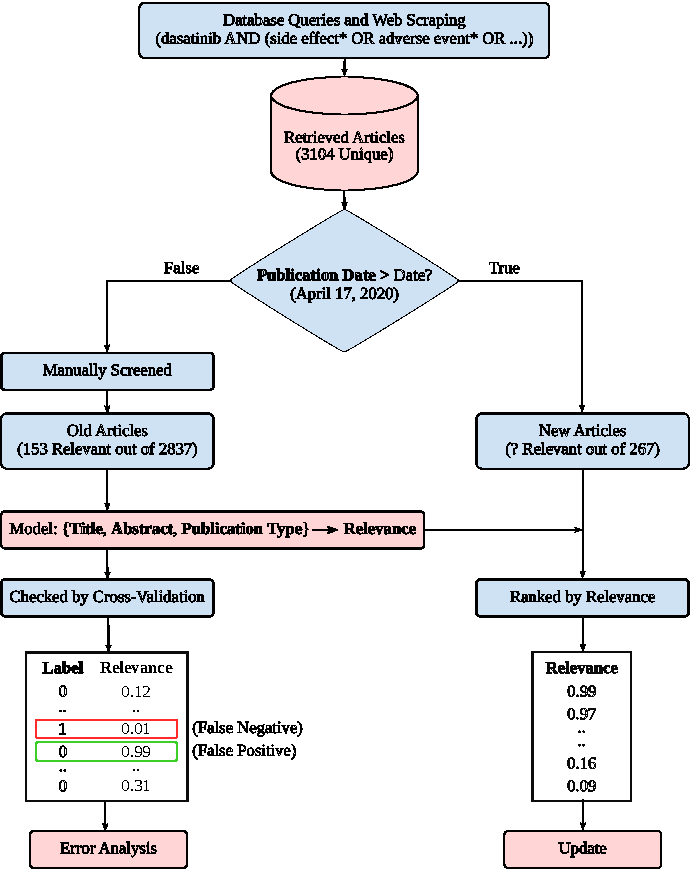
\includegraphics[width=\linewidth]{../diagrams/general-overview/general-overview-crop.pdf}
    \captionof{figure}{General overview of proposed framework.}
    \label{fig:overview}
\end{center}%
\vspace{4mm}
}]%
\saythanks

\begin{tikzpicture}[remember picture,overlay]
\node[align=left,text=black] at ([yshift=1em]current page text area.north west)%
{ 
\hspace{46mm} \footnotesize{\texttt{TECHNICAL REPORT 10 March 2021}}\\
\hspace{46mm} \footnotesize{\texttt{DOI: 10.5281/zenodo.4593957}}%
};
\end{tikzpicture}%

\begin{abstract}
{This report describes the initial results of a research project to develop a machine learning framework to semi-automate citation screening in systematic reviews and meta-analyses. It was developed and evaluated in context of aging and longevity research studies. We conducted experiments on dataset related to a specific risk-benefit analysis. Empirical results show that by using the proposed system, reviewers save an average of around 60\% of screening work compared to unaided screening to identify 95\% of relevant papers. The logistic regression model used in our framework is one of the simplest machine learning models and very efficient to train. The resulting model is used for the update of the analysis, thereby offering an opportunity to reduce the reviewers workload. In addition, we use the results from cross-validation procedure to help identify potential screening errors made. We outline the framework and how it can be used in similar screening practices. The software  is open sourced with dataset freely available{\footnote{\url{https://github.com/markolalovic/longevity-research-screening/}}}.
}
\end{abstract}

\keywords{Automated screening, Literature prioritization, Machine learning, Text mining, Software}

% copyright
© The Author 2021 This work is licensed under a Creative Commons Attribution 4.0 International license\footnote{\url{https://creativecommons.org/licenses/by/4.0/}}.

\newpage
\section{Introduction}
  
A systematic review typically addresses a specific clinical question by collecting and analyzing data from all the relevant and unbiased set of studies. Citation screening is the first yet tedious task of narrowing down the large set of citations retrieved via a broad database query to those relevant for the review. Machine learning (ML) refers to algorithms that can learn from and make predictions on data by building statistical models.

\begin{figure*}[ht]
\centering
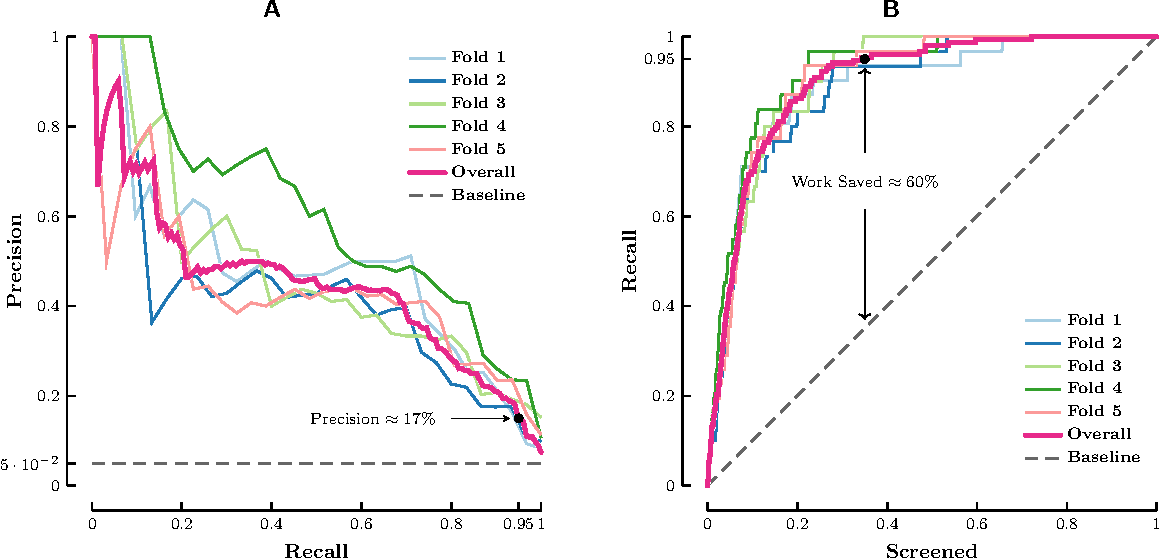
\includegraphics[width=1\textwidth]{../figures/performance-evaluation/combined/performance-evaluation-crop.pdf}
\caption{Visualized results of 5-fold cross-validation for D\&Q Analysis.}
\label{fig:performance-evaluation}
\end{figure*}

{\bf Related Work.} The work in (semi)-automation of citation screening is active and diverse. Wallace et al.~\cite{semi-automated} developed a semi-automated citation screening algorithm for systematic reviews of biomedical literature. Bannach-Brown et al.~\cite{animal-studies} described their approaches to aid citation screening for a systematic review of preclinical animal studies. Howard et al.~\cite{swift-workbench} deployed a general software system that automate the required methodologies called ``SWIFT-Review". Przybyła et.al~\cite{robot-analyst} introduced a web-based software system called ``RobotAnalyst". O’Mara-Eves et al.~\cite{mining-review} performed a systematic review of current approaches. They concluded, on one side, that the use of these tools to automatically eliminate studies is promising but should be used cautiously, since the reviews are at risk of limiting their review to such a degree that the validity of their findings is questionable. On the other side, using them in order to prioritize the order in which papers are screened should be considered safe and ready for use in actual reviews. However, the use of these tools varies greatly across disciplines. To date, no use of any tools related to automating (or semi-automating) the screening process of systematic reviews or meta-analyses of aging and longevity research was reported. More developmental work is needed and more validation of these methods needs to be performed before all systematic review teams can take advantage of these tools.
 
The aim of this work is to develop an easy to use tool that can be used in the screening stage of systematic reviews or meta-analyses of aging and longevity research studies to reduce the reviewers workload (and screening error). Here, we present a simple ML framework that enables us to connect the data and models, evaluate the performance and deploy and interpret the results in the form of interactive tables accessible from a browser.

{\bf General Overview}. Query databases of biomedical research publications using a provided list of search terms. Process documents (consisting of metadata, title and abstract) using natural language processing tools and save the results into a local database. Split the documents in the following two sets. First set consists of {\it labeled documents}, meaning that each document is manually screened and assigned a label (1 = relevant, 0 = not relevant) based on reviewers decision. The set of labeled documents is used to train a statistical model. The fitted model estimates the probability called {\it relevance score}, that a given document is relevant. Apply the model to the second set of unlabeled documents to estimate their relevance scores and rank them according to their estimated relevance scores. In addition, using the cross-validation procedure, assign relevance scores to all labeled documents to help identify any false labeled documents. Export the results in the form of interactive tables to a web application. These steps are visualized in Figure~\ref{fig:overview}.

We conducted experiments on dataset related to Dasatinib and Quercetin Senolytic Therapy Risk-Benefit Analysis (D\&Q Analysis). The analysis is part of ``Rejuvenation Now" non-profit initiative that: ``seeks to continuously identify potential rejuvenation therapies and systematically evaluate their risks, benefits, and associated therapeutic protocols to create transparency" published by Forever Healthy Foundation\footnote{\url{https://brain.forever-healthy.org/display/EN/}}. 
Here, the split was based on publication date of review. We used labeled documents from existing systematic review. The resulting model was then applied to new documents retrieved in subsequent search to be used for an update of the original review. In our approach we focused on maximizing the recall. {\it Recall} (also known as {\it sensitivity}) is the fraction of relevant documents that are also retrieved as relevant by the system. For a formal definition of recall, other key measures and curves, see Section~\ref{sec:evaluation}.

\begin{table*}[ht]
\centering
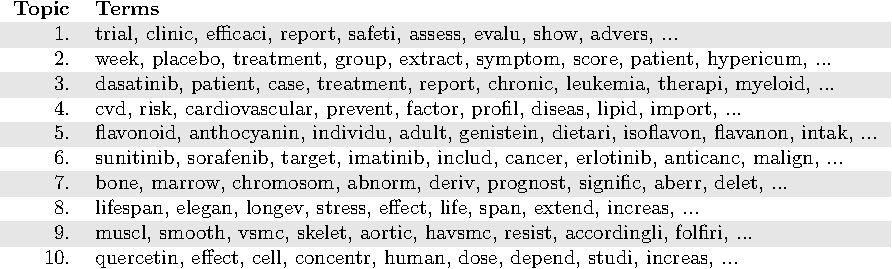
\includegraphics[width=.85\textwidth]{../tables/topics/topics-crop.pdf}
\caption{Terms of the first 10 extracted topics.}
\label{tab:topics}
\end{table*}


{\bf Results.} The following values are estimates based on 153 labeled documents using 5-fold cross-validation procedure. For more details, see Section~\ref{sec:eval-results}. The empirical results show that the proposed system can identify 95\% of relevant documents with precision 17\%; see Figure~\ref{fig:performance-evaluation}A. This means that only around 17\% of identified documents are actually relevant. The performance of the system is still reasonable, since the reviewers have to screen only around 35\% of retrieved documents on average. This saves them on average around 60\% of work comparing to screening documents in random order where they would need to screen 95\% of documents on average to achieve the desired 95\% recall; see Figure~\ref{fig:performance-evaluation}B.

\section{Methods}

We describe the methodology and how it was applied to Dasatinib and Quercetin Senolytic Therapy Risk-Benefit Analysis (D\&Q Analysis).

\subsection{Data}
We first query the publicly available PubMed (MEDLINE) database using pymed API. This can be easily expanded to other sources, for example to Cochrane Library. The search terms for D\&Q Analysis were devised by Forever Healthy foundation. Additionally, we scrape some data directly from websites of journals or clinical trials (ClinicalTrials.gov) using chromedriver in Python. The retrieved data is saved into local MySQL database. For each article we save its url (where it was retrieved from), publication date, publication types, title and abstract. For papers that were manually screened, we also save the assigned label (1 = relevant, 0 = not relevant). 

We retrieved 2837 potentially relevant papers for D\&Q Analysis. Of these, only 153 papers were labeled as relevant. The prevalence of relevant class in this dataset is approximately 5\%. This means that this dataset is highly imbalanced and requires more complex statistical modeling and evaluation.

\subsection{Pre-Processing} 
For the purposes of statistical modeling, the retrieved data is processed in the following way. The words in title and abstract are filtered based on part-of-speech tags to remove low information words such as english stop words. The remaining words are then reduced to their base forms using lematization to improve the statistical modeling performance. Both of this text processing steps are done using spaCy Python library. Lastly, we append the prefix \texttt{title} to words in title to separate them from words in abstract. Combined title, abstract and publication types of each paper is called {\it document}.

\begin{figure*}[ht]
\centering
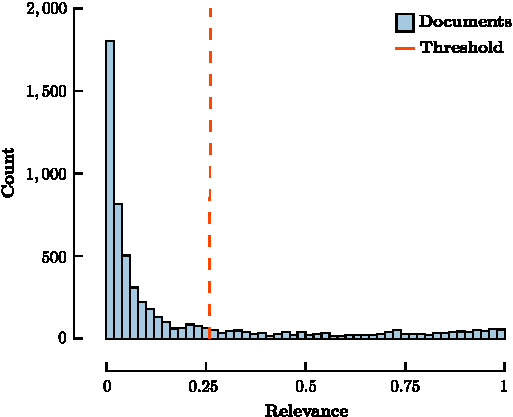
\includegraphics[width=0.55\textwidth]{../figures/threshold-selection/threshold-selection-crop.pdf}
\caption{The selected cut-off threshold for D\&Q Analysis was 0.26 where the binary classifier achieved 95\% recall.}
\label{fig:threshold-selection}
\end{figure*}

\subsection{Feature Extraction} 
Each document $d$, is represented by a vector $X^{d}$. Components of $X^{d}$ are called {\it features} and denoted by $X_{*}^{d}$ where * stands for the name of the feature. First, two sets of simple binary features are created. First set of binary features is based on the provided list of search terms to construct a query (e.g.: \texttt{dasatinib}, \texttt{senolytic}, \texttt{senescent}, ...). For each search term $st$, the value of $X_{st}^{d}$ is 1, if $st$ appears in the document $d$, otherwise the value is 0. Second set of binary features is based on possible publication types (e.g.: \texttt{case report}, \texttt{clinical trial}, \texttt{review}, ...). For each publication type $pt$, the value of $X_{pt}^{d}$ is 1, if $pt$ appears in the document $d$, otherwise the value is 0.

The next set of features is based on bag-of-words representation of {\it $n$-grams}. These are contiguous sequences of $n$ words called {\it terms} (e.g.: \texttt{chronic myeloid}, \texttt{adverse event}, \texttt{tyrosine kinase}, ...). Here, we allow for 2-grams (pairs of words). From this representation, Term Frequency - Inverse Document Frequency (TF-IDF) matrix is constructed. The matrix consists of term scores. The terms which help to distinguish between documents have higher scores. For each term $t$, the value of $X_{t}^{d}$ is TF-IDF score of the term $t$ in document $d$:

$$
X_{t}^{d}=\text{TF-IDF}_{t, d}.
$$

For the last set of features, the latent Dirichlet allocation (LDA) topic model is constructed using MALLET library. See Table~\ref{tab:topics} for examples of extracted topics. For each topic $u$, the value of $X_{u}^{d}$ is the probability that document $d$ belongs to the topic $u$:

$$
X_{u}^{d}=\text{Pr}(\text{document $d$ belongs to the topic $u$}).
$$

Finally, the features are standardized to have zero mean and unit variance:
$$
X^{d} \coloneqq \frac{ X^{d} - \overline{X^{d}} }{ \sigma_{X^{d}} }.
$$

\subsection{Model}
Given the labeled documents, we build a logistic regression model from scikit-learn library in Python. The logistic regression model used in our framework is one of the simplest machine learning models and very efficient to train. The model estimates the conditional probability, called {\it relevance score}, that a given document $d$ is relevant given feature vector $X^{d}$:

$$
\text{Pr}(\text{$d$ is relevant} | X^{d})
$$

To avoid over-fitting, we use L1-regularization parameter $C$. For tuning parameter $C$ we place more emphasis on recall by using recall scorer. Model is fitted using Liblinear solver with balanced class weights to improve the recall. For D\&Q Analysis the value of L1-regularization parameter $C$ was selected to be around $0.02$. The support, or the number of features with non-zero weights in the model, was around 28. These are average values across the folds when using cross-validation procedure explained next.

\begin{table*}[ht]
\centering
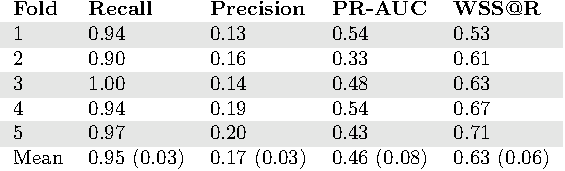
\includegraphics[width=0.5\textwidth]{../tables/evaluation-results/evaluation-results-crop.pdf}
\caption{Summarized results of 5-fold cross-validation for D\&Q Analysis.}
\label{tab:eval-results}
\end{table*}

\subsection{Performance Evaluation} \label{sec:evaluation}

% testing procedure
Evaluation is done using the standard testing procedure called {\it k-fold cross-validation} for $k=5$. This involves randomly partitioning the set of documents into 5 complementary subsets called {\it folds} of nearly equal size. Stratified sampling is used for partitioning to ensure that the folds have similar proportion of relevant documents. Then over 5 iterations, the model is fitted on 4 folds, called {\it train set}, and validated on the remaining fold, called {\it test set}. Each fold is used once as a test set. Thus, every document is part of the test set once and is assigned the relevance score. The distribution of relevance scores for all the documents are shown in Figure~\ref{fig:threshold-selection}.

These relevance scores are then compared to human assigned labels in the following way. Documents with relevance score higher than selected cut-off threshold are classified as relevant. All other documents are classified as not relevant. The result is a binary classifier. For D\&Q Analysis the selected threshold was 0.26 where the binary classifier achieved 95\% recall. For a particular document, the four possible outcomes of comparing the classification result with human assigned label are defined in the following table:

\begin{table}[H]
\centering
\resizebox{0.27\textwidth}{!}{
\noindent
\renewcommand\arraystretch{1.5}
\setlength\tabcolsep{4pt}
\begin{tabular}{c >{\bfseries}r @{\hspace{0.7em}}c @{\hspace{0.4em}}c @{\hspace{0.7em}}l}
  \multirow{10}{*}{\rotatebox{90}{\parbox{5cm}{\bfseries\centering Labeled as relevant}}} & 
    & \multicolumn{2}{c}{\bfseries Classified as relevant} & \\
  & & \bfseries Yes & \bfseries No \\
  & Yes & \MyBox{\it True}{\it positive} & \MyBox{\it False}{\it negative} \\[2.4em]
  & No & \MyBox{\it False}{\it positive} & \MyBox{\it True}{\it negative}
\end{tabular}
}
\end{table}

The number of all true positives out of all the documents is denoted by $TP$. Similarly for other outcomes, the numbers of outcomes out of all the documents are denoted by $FN, FP$ and $TN$. Performance was assessed using four statistical measures of binary classifier performance. {\it Precision} $P$ is the fraction of documents labeled as relevant among documents classified as relevant:
$$
P = \frac{TP}{TP + FP}
$$
{\it Recall} $R$ (also known as {\it sensitivity}) is the fraction of documents labeled as relevant that were also classified as relevant:
$$
R = \frac{TP}{TP + FN}
$$
There is an inverse relationship between precision and recall. Depending on the selected threshold, it is possible to increase one at the cost of reducing the other. For example, by selecting the threshold of 0, we classify all documents as relevant and achieve maximum recall of 1 at the cost of precision, which is the proportion of documents labeled as relevant among all the documents (which is approximately 0.05 in our case). {\it Precision-recall curve} illustrates this trade off by plotting precision and recall as a function of selected cut-off threshold. {\it PR-AUC} is the area under the precision-recall curve. It is a performance measure used to compare classifiers or estimate the average precision of a classifier.

We can also order the documents based on their relevance scores and screen the documents in this order. We can visualize the ranking performance by plotting recall as a function of proportion of documents screened. {\it Work Saved over Sampling} $WSS@R$ is the reduction of documents that need to be screened compared to a random ordering of the documents to achieve a level of recall $R$:

$$
WSS@R = \frac{TN + FN}{N} - (1 - R)
$$

Here $N$ denotes the number of all documents:
$$
N = TP + FN + FP + TN
$$

\begin{figure*}[ht]
\centering
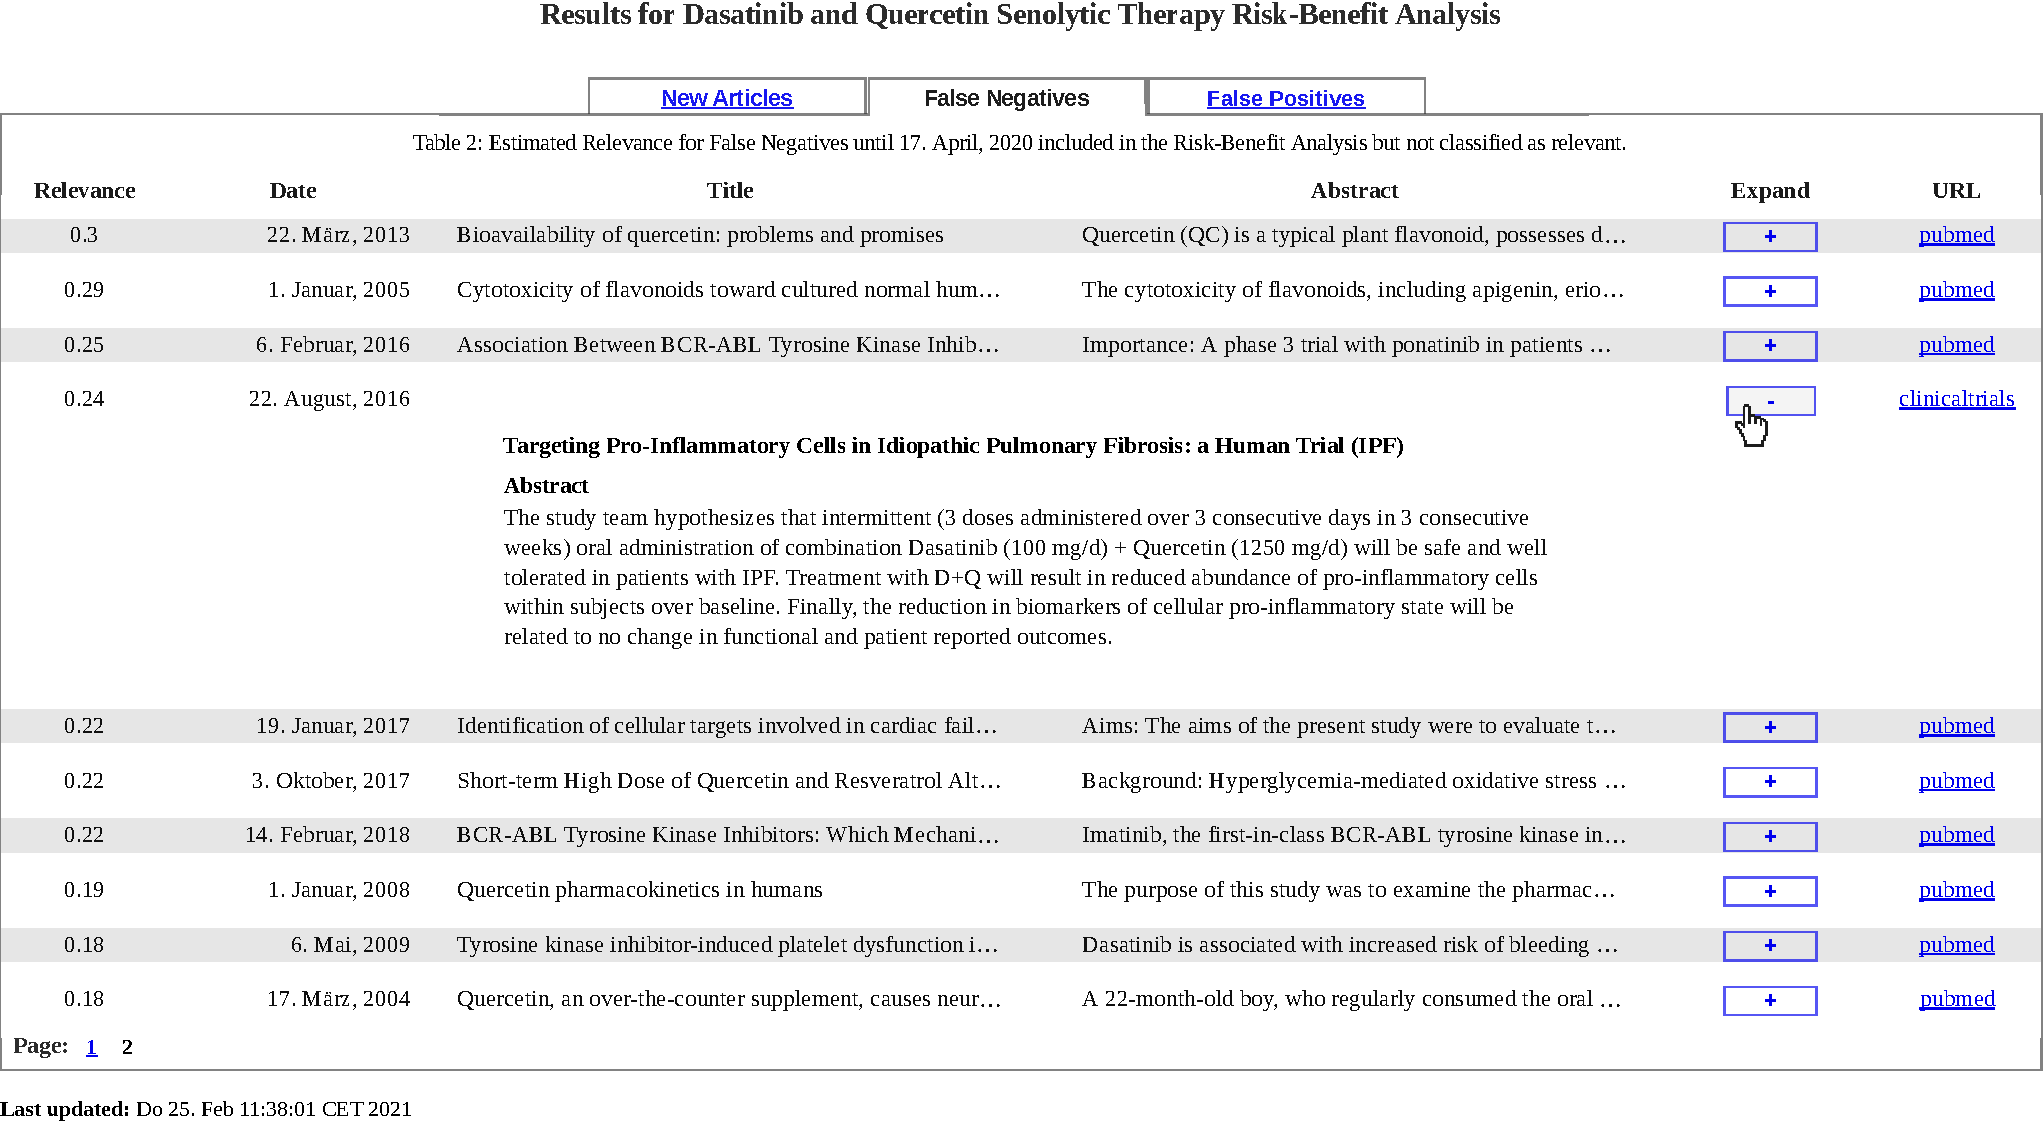
\includegraphics[width=1\textwidth]{../tables/export-tables/export-tables-crop.pdf}
\caption{Interactive tables of exported documents for D\&Q Analysis.}
\label{fig:export}
\end{figure*}

\subsection{Evaluation results} \label{sec:eval-results}
The results for each fold of 5-fold cross-validation for D\&Q Analysis are summarized in Table~\ref{tab:eval-results} and visualized in Figure~\ref{fig:performance-evaluation}. For selected cut-off threshold of 0.26 the estimated average performance across all 5 folds ($\text{mean} \pm \text{sd}$) was:
\begin{align*}
P &= 0.17\pm 0.03 \\
R &= 0.95\pm 0.03 \\
WSS@R &= 0.63\pm 0.06
\end{align*}

We get very similar estimates from combined confusion matrix across all folds since we are using stratified sampling. We can interpret this results in the following way. In a set of new unlabeled documents that are assigned the relevance score of more than 0.26, we can expect the following: 
\begin{itemize}
\item around 17\% of documents in this set are relevant;
\item around 95\% of all the relevant documents are in this set;
\item around 60\% of screening work is saved if screening only this set comparing to random order screening.
\end{itemize}

\subsection{Export}
We exported 267 retrieved documents from new papers published after the publication of D\&Q Analysis (April 17, 2020) sorted by relevance scores that were assigned by the final model trained on all the labeled documents to be used for the update of analysis. In addition, we exported all false negatives and false positives from labeled documents sorted by assigned relevance scores to identify potential screening errors made in the original review. 

The result are 3 interactive tables of exported documents, shown in Figure~\ref{fig:export} and accessible online\footnote{\url{https://markolalovic.com/longevity-research-screening/}}. The user can expand each document to see the title and abstract of the corresponding paper or follow the provided url.

\subsection{Conclusion}
In this work, we have introduced a simple machine learning framework that can be used in the screening stage of systematic reviews or meta-analyses. We applied it to a particular dataset related to a specific risk-benefit analysis published by Forever Healthy Foundation. The empirical results show that by using the proposed framework, we are able to identify 95\% of relevant documents from a set of all documents retrieved via a broad database query. We estimated that reviewers can save an average of around 60\% of screening work comparing to unaided screening to achieve this result. The proposed system can already be used to prioritize the order in which papers are screened. Or as a "second screener" based on exported documents that the system falsely classified as relevant, to help identify potential screening errors made.

More development is needed and validation on different datasets needs to be performed before using this framework to automatically remove studies for a review. The features should reflect what reviewers are looking for in a specific systematic review when deciding which paper is relevant. For example, they may be looking for effect size or try to detect large deviations in effect size. More collaboration with systematic review teams is needed to create such features. In the future, we would like to extend this work and evaluate it on different datasets.

\bibliographystyle{ieeetr}
\bibliography{main}

\end{document}

